\chapter{Simulation Framework}
\label{chap:simulation}

This chapter describes the framework used to simulate realistic AGN multiband light curves in the LSST \textit{ugriz} bands. The simulation is based on the damped random walk (DRW) model, whose parameters are assigned using empirical wavelength-dependent scaling relations, and implemented using the \textsc{EzTao} Gaussian process library \parencite{Yu2022Extao}.

%Gaussian processes with an exponential autocorrelation fall into this class of stochastic models that have fast algorithms for computing their likelihood function (Rybicki & Press 1995; Koz lowski et al. 2010). This particular process is known as both a first order continuous-time autoregressive process (CAR(1)) or an Ornstein-Uhlenbeck process , and was introduced by Kelly et al. (2009) as a model for quasar optical light curves.

\section{The Vera C. Rubin Observatory LSST}
\label{sec:LSST}
% we chose the lsst-like simulations because ...

\section{Damped Random Walk}
\label{sec:DRW}

The simplest stochastic model consistent with the observed AGN PSD properties is the \textit{damped random walk} (DRW), also known as a first-order continuous autoregressive process, CAR(1), or Ornstein-Uhlenbeck process \parencite{Kelly2009ThermalFluc}. It is described by the stochastic differential equation:

\begin{equation}
    \label{eq:DRW}
    df(t) = -\frac{f(t)}{\tau_\mathrm{DRW}}\,dt + \sigma_\mathrm{DRW}\sqrt{dt}\,\epsilon(t),
\end{equation}

where $\tau_\mathrm{DRW}$ is the damping (or characteristic) timescale, $\sigma_\mathrm{DRW}$ is the asymptotic variability amplitude, and $\epsilon(t)$ is a white noise process. The DRW has an exponential autocorrelation function:

\begin{equation}
    \label{eq:DRW_ACF}
    \mathrm{ACF}(\Delta t) = \exp\left(-\frac{|\Delta t|}{\tau_\mathrm{DRW}}\right),
\end{equation}

corresponding to a PSD of the form $P(\nu) \propto \nu^{-2}$ at high frequencies, flattening to white noise below the break frequency $\nu_b = 1/(2\pi\tau_\mathrm{DRW})$. In the structure function representation, the DRW produces a power-law rise with slope $\gamma = 0.5$ on short timescales ($\Delta t \ll \tau_\mathrm{DRW}$), flattening to a constant value set by $\sigma_\mathrm{DRW}$ above the characteristic timescale (Figure~\ref{fig:KozlowskiDRW}; \cite{Kozlowski2016SF}). The DRW has been shown to provide a good statistical description of optical AGN light curves \parencites{Kelly2009ThermalFluc}{Kozlowski2010DRW}{MacLeod2010ScalRel}, with $\tau_\mathrm{DRW}$ found to correlate with black hole mass and luminosity, consistent with the physical picture developed in Chapter~\ref{chap:variability}.

\begin{figure}[t]
    \centering
    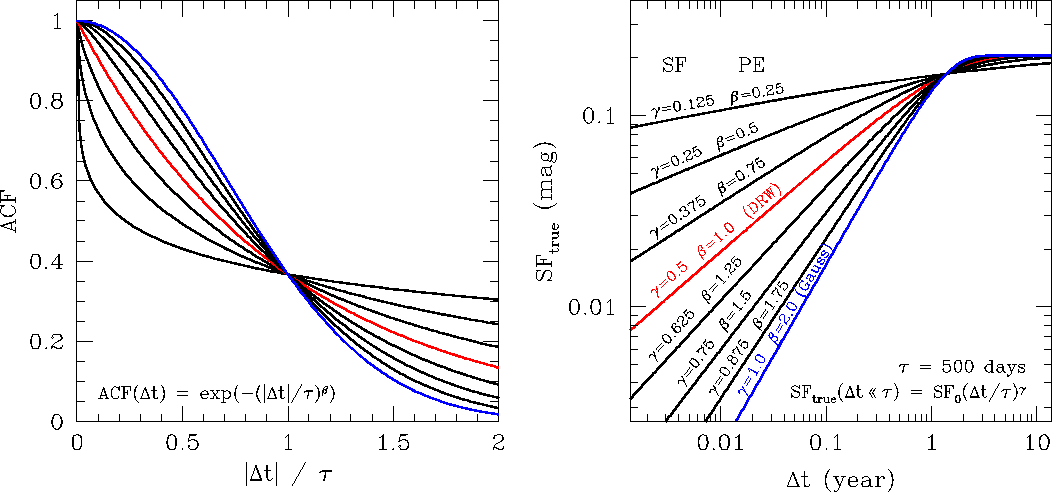
\includegraphics[width=\textwidth]{assets/3_figures/Kozlowski2016.pdf}
    \caption[Connection between exponential ACFs and structure functions for different stochastic models]{\label{fig:KozlowskiDRW} Left: Exponential autocorrelation functions $\mathrm{ACF}(\Delta t) = \exp(-(|\Delta t|/\tau)^\beta)$ for different values of $\beta$. Right: The corresponding structure functions. The DRW model ($\beta = 1$, red) produces a SF with slope $\gamma = 0.5$ on timescales $\Delta t \ll \tau$, flattening above the characteristic damping timescale. Adapted from \cite{Kozlowski2016SF}.}
\end{figure}

The DRW is the simplest member of the broader family of continuous autoregressive moving average (CARMA) models \parencite{Kelly2014CARMA}, corresponding to the special case CARMA$(1,0)$. More flexible CARMA$(p,q)$ processes can reproduce a wider range of PSD shapes; in particular, the CARMA$(2,1)$ process, also known as the damped harmonic oscillator (DHO), has been shown to provide superior fits to observed AGN light curves compared to the DRW \parencite{YuEzTao2025}. The simulation framework described here assumes a DRW process for the underlying variability, though the implementation supports more general CARMA kernels.

\section{Multiband Light Curve Simulation}
\label{sec:MultibandSim}

\subsection{DRW Parameters and MacLeod Scaling Relations}
\label{ssec:MacLeod}

The DRW parameters $\tau_\mathrm{DRW}$ and $\sigma_\mathrm{DRW}$ depend on the observing wavelength, black hole mass, and luminosity. Following \textcite{MacLeod2010DRW}, the wavelength dependence can be expressed as power-law scaling relations:

\begin{equation}
    \label{eq:MacLeod}
    \tau_\mathrm{DRW} \propto \lambda^{0.17}, \qquad \sigma_\mathrm{DRW} \propto \lambda^{-0.479},
\end{equation}

where $\lambda$ is the effective wavelength of the observing filter. These relations imply that redder bands have slightly longer damping timescales and lower variability amplitudes than bluer bands, consistent with the wavelength dependence of AGN variability discussed in Chapter~\ref{chap:variability}.

In the simulation framework, a \textit{driver band} is defined as the reference band from which the DRW parameters of all other bands are derived via Equation~\ref{eq:MacLeod}. The driver band parameters ($\tau_\mathrm{DRW}^g = 100$ days, $\sigma_\mathrm{DRW}^g = 0.112$ mag) are taken as fiducial values representative of typical quasar optical variability \parencite{YuEzTao2025}, with the $g$ band chosen as the reference. The parameter space explored in this work follows \textcite{YuEzTao2025}:

\begin{equation}
    \tau_\mathrm{DRW} \in [0.01, 500] \text{ days} \quad \text{(log-uniform)}, \qquad \sigma_\mathrm{DRW} \in [0.02, 0.2] \text{ mag} \quad \text{(log-uniform)}.
\end{equation}

\subsection{EzTao Implementation}
\label{ssec:EzTao}

"EzTaoX models AGN UV/optical stochastic variability as a Gaussian processes (GP), a method commonly adopted in AGN variability analysis (e.g. Press et al. 1992; Kelly et al. 2009; Kozłowski et al. 2010; Wilkins 2019; Griffiths et al. 2021; Yu et al. 2022; Stone et al. 2022; Zhang et al. 2023; McLaughlin et al. 2024). Since the flux light curves of accreting compact objects typically follow a lognormal distribution (e.g., Uttley & McHardy 2001; Gaskell 2004; Giebels & Degrange 2009; MacLeod et al. 2012; De Cicco et al. 2022), we emphasize that GP modeling is best applied to magnitude light curves, which follow a Gaussian distribution" 

\subsection{Noise Model}
\label{ssec:Noise}

Observational noise is simulated by adding Gaussian random values drawn from $\mathcal{N}(0, \sigma_\mathrm{LSST}^2)$ to each flux measurement, where $\sigma_\mathrm{LSST} = 0.01$ mag is the expected LSST single-visit photometric uncertainty\footnote{\url{https://rubinobservatory.org/for-scientists/rubin-101/key-numbers}}.

\subsection{Sampling Strategy}
\label{ssec:Sampling}

The simulation supports two modes: a single-band driver light curve (\texttt{makeDriver}), which generates a single DRW realisation at the reference band parameters on a uniform time grid with step $\Delta t$ up to a maximum baseline $t_\mathrm{max}$; and a multiband mode (\texttt{makeMultiband}), which generates correlated light curves in all requested bands simultaneously using the wavelength-scaled parameters. A sparse sampling mode (\texttt{makeSparse}) is also implemented to mimic realistic LSST observing cadences by subsampling the uniform grid with gaps and irregular spacing.


% before we interpolated the original light curve into the new observed times, now we resimulate the process

% For each realisation we draw the number of attempted observations N_obs uniformly in [70, 200] and the gap fraction uniformly in [0.1, 0.5]. Gaps are laid out as disjoint windows wholly inside the baseline, so the removed fraction is exact; individual gap widths are drawn from a uniform simplex and therefore span roughly 0.1–4 τ_DRW.


%t_obs  = self.makeSparse(...)                      # cadence first
%t_all  = np.union1d(self.t_true, t_obs)            # union grid
%t_all, y_all = self.makeDriver(t_all, lc_seed)     # ONE simulation
%y_true      = y_all[searchsorted(t_all, self.t_true)]   # slice truth
%y_obs_clean = y_all[searchsorted(t_all, t_obs)]         # slice obs
%y_obs, yerr = self.addGNoise(y_obs_clean, ...)     # noise last

\section{Simulation Regime}
\label{sec:regime}
Simulation regime. Gap-filling difficulty is controlled by a single dimensionless quantity, Δt/τ_DRW, because a DRW forgets as exp(−Δt/τ). We therefore quote our simulation parameters in units of τ rather than in days. With a three-year baseline (t_max = 1095 d), N_obs = 130 attempted epochs, a gap fraction of 0.35 distributed over three windows, and the Yu et al. (2025) fiducial g-band driver (τ_DRW = 100 d, σ_DRW = 0.112 mag), the mean cadence is 8.4 d = 0.084 τ, the mean gap is 128 d = 1.28 τ, and the baseline is 10.9 τ. Consecutive epochs are therefore strongly correlated while the gaps straddle the decorrelation scale — the regime in which reconstruction is neither trivial nor impossible. (The mean cadence is independent of the gap fraction, since gaps remove observing time and epochs in the same proportion; note also that because the epochs are drawn uniformly the spacings are exponentially distributed, so the median cadence is ln2 ≈ 0.69 times the mean.)
Two thresholds bracket this range. Both appear in the literature as biases on τ_DRW recovery — τ is underestimated when the baseline is shorter than ~10 τ (Kozłowski 2017), and overestimated when τ is less than ~5 times the mean cadence (Hu et al. 2024) — but they matter here for a different reason: they delimit where a gap carries information at all. Below the cadence threshold, consecutive epochs are uncorrelated and no interpolation is possible, so the model can only return the prior; above the baseline threshold, the driver barely decorrelates over the observing window and every gap is trivially interpolable. This is also why we fix τ_DRW = 100 d rather than adopting the LogUniform(0.01, 500) d range of Yu et al. (2025): that range was chosen to probe τ-recovery across its failure regimes, whereas here roughly 80\% of it would produce degenerate light curves. Should τ diversity be introduced later, LogUniform(30, 300) d spans the informative range at this baseline and cadence.